Para a ShuffleNet, não verificou-se a necessidade de uma busca em \emph{grid} entre os hiperparâmetros, considerando os bons resultados apresentados pela MobileNet e pela semelhança existente entre estas CNNs. Entretanto, para demonstrar a eficiência da ShuffleNet, foram escolhidos hiperparâmetros de maneira \emph{ad hoc}, baseando-se apenas naqueles hiperparâmetros que demonstraram um bom desempenho nas arquiteturas anteriores. Por conseguinte, foram treinados dois modelos com os mesmos hiperparâmetros, um para cada abordagem, os quais obtiveram as métricas dispostas na Tabela \ref{tab:shufflenet}. O histórico de \emph{loss} e acurácia durante o ajustamento dos modelos estão retratados na Figura \ref{fig:treinamento-shufflenet}.

\begin{table}[h!]
\centering
\caption{Detalhamento dos modelos obtidos com a arquitetura ShuffleNet para cada uma das abordagens consideradas neste trabalho.}
\label{tab:shufflenet}
\resizebox{\textwidth}{!}{\begin{tabular}{ccccccc}
\toprule
\textbf{Abordagem} & \textbf{Otimizador} & \textbf{\emph{Patience}}  & \textbf{Função de Ativação} & \textbf{Acurácia} & \textbf{F-Score} & \textbf{EER} \\
\midrule
Abordagem A & RMSprop & 15 & ReLU & $0.9404$ & $0.9004$ & $7.5400$ \\
Abordagem B & RMSprop & 15 & ReLU & $0.8345$ & $0.7705$ & $23.8151$\\
\bottomrule
\end{tabular}}
\end{table}
    
\begin{figure}[H]
\centering
\caption{Histórico de \emph{loss} e acurácia durante o treinamento dos modelos obtidos com a arquitetura ShuffleNet.}
\label{fig:treinamento-shufflenet}
\subfloat[\emph{Loss} durante treinamento da rede ShuffleNet para a abordagem A.\label{subfig:shufflenet-a-loss}]{%
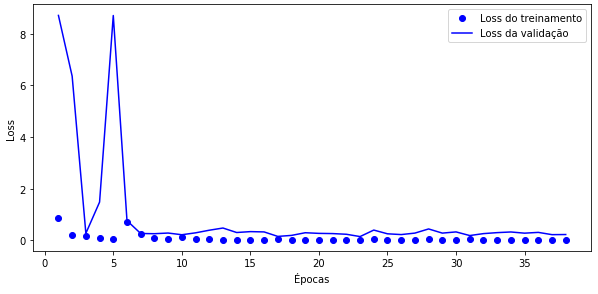
\includegraphics[width=0.47\textwidth]{imgs/shufflenet-a-loss}
}
\hfill
\subfloat[Acurácia durante treinamento da rede ShuffleNet para a abordagem A.\label{subfig:shufflenet-a-acc}]{%
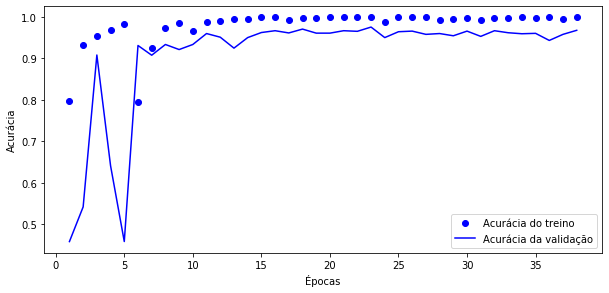
\includegraphics[width=0.47\textwidth]{imgs/shufflenet-a-acc}
}
\hfill
\subfloat[\emph{Loss} durante treinamento da rede ShuffleNet para a abordagem B.\label{subfig:shufflenet-b-loss}]{%
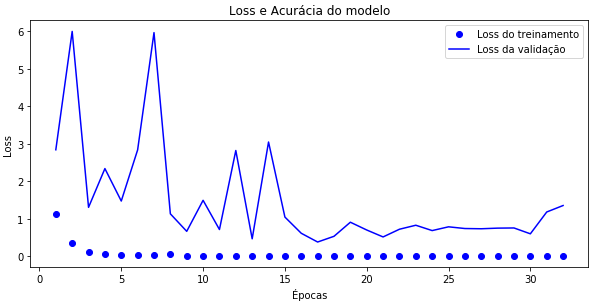
\includegraphics[width=0.47\textwidth]{imgs/shufflenet-b-loss}
}
\hfill
\subfloat[Acurácia durante treinamento da rede ShuffleNet para a abordagem B.\label{subfig:shufflenet-b-acc}]{%
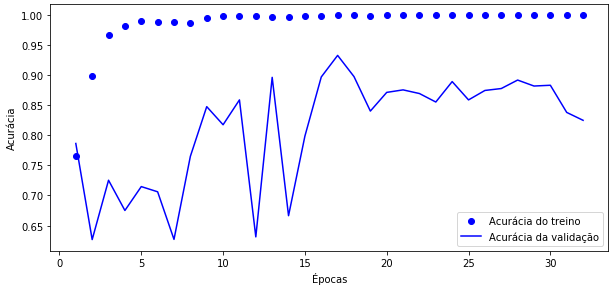
\includegraphics[width=0.47\textwidth]{imgs/shufflenet-b-acc}
}
\end{figure}

Ao analisar as métricas obtidas por esta arquitetura, observa-se um desempenho inferior ao observado pelas arquiteturas anteriores, isto se deve, presumivelmente, à subexploração dos hiperparâmetros possíveis, principalmente considerando que modelos da arquitetura MobileNet não expostos neste trabalho, por exemplo, obtiveram métricas similares ou inferiores.

As matrizes de confusão destes modelos, dispostas na Figura \ref{fig:matrizes-shufflenet}, mostram uma grande quantidade de falsos negativos e nenhum falso positivo para a abordagem A. Este cenário mostra uma grande eficiência do modelo em detectar assinaturas falsificadas. Na matriz da abordagem B, por outro lado, o quantitativo de falsos positivos foi por volta de $40\%$ maior do que a quantidade de falsos negativos. Esta quantidade de erros cometido pelo classificador é refletida diretamente na métrica EER, a qual possui o maior valor encontrado entre os modelos expostos até então.
    
\begin{figure}[h]
    \centering
    \caption{Matrizes de confusão dos modelos obtidos com a arquitetura ShuffleNet.}\label{fig:matrizes-shufflenet}
    \subfloat[ShuffleNet com a abordagem A\label{subfig:matriz-shufflenet-a}]{%
    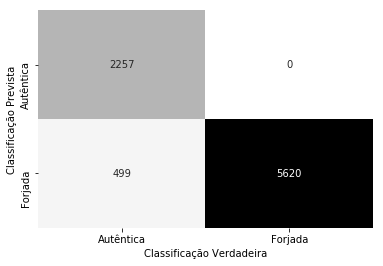
\includegraphics[width=0.47\textwidth]{imgs/matriz-shufflenet-a}
    }
    \hfill
    \subfloat[ShuffleNet com a abordagem B\label{subfig:matriz-shufflenet-b}]{%
    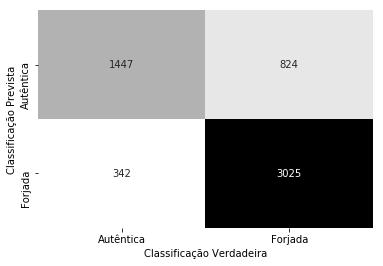
\includegraphics[width=0.47\textwidth]{imgs/matriz-shufflenet-b}
    }
\end{figure}

Ao que tudo indica, a utilização da arquitetura ShuffleNet, associada a uma busca de bons hiperparâmetros, pode ser bem aproveitada para a tarefa de aprendizado apresentada neste trabalho, observando principalmente as necessidades e especificações de um sistema em um cenário de aplicação real.